% Componentes contravariantes (paralelas) y covariantes (perpendiculares) — libro fig. 5.6
\documentclass[border=5pt]{standalone}
\usepackage{tikz}
\usetikzlibrary{arrows.meta, calc}
\begin{document}
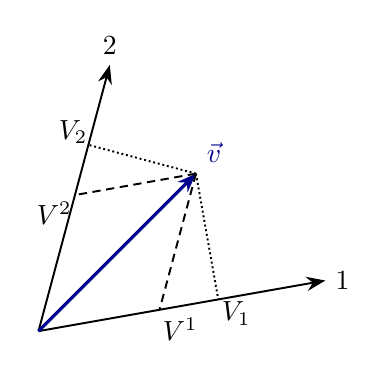
\begin{tikzpicture}[>={Stealth[length=2.4mm]}, line width=0.7pt]
  \coordinate (O) at (0,0);
  \coordinate (V) at (2.0,2.0);
  % ejes inclinados
  \draw[->] (O)--(10:3.7) node[right]{$1$};
  \draw[->] (O)--(75:3.5) node[above]{$2$};
  % vector v
  \draw[->, line width=1.2pt, blue!55!black] (O)--(V) node[above right]{$\vec v$};
  % CONTRAVARIANTES: proyección paralela a los ejes (discontinuo)
  \draw[densely dashed] (V)--(1.537,0.271); \node[below right] at (1.45,0.30){$V^1$};
  \draw[densely dashed] (V)--(0.463,1.728); \node[left] at (0.55,1.5){$V^2$};
  % COVARIANTES: proyección perpendicular a los ejes (punteado, con ángulo recto)
  \draw[densely dotted] (V)--(2.283,0.403);
  \draw[densely dotted] (V)--(0.634,2.366);
  \node[below right] at (2.2,0.5){$V_1$};
  \node[above left] at (0.75,2.25){$V_2$};
\end{tikzpicture}
\end{document}
